% Options for packages loaded elsewhere
\PassOptionsToPackage{unicode}{hyperref}
\PassOptionsToPackage{hyphens}{url}
\PassOptionsToPackage{dvipsnames,svgnames,x11names}{xcolor}
%
\documentclass[
  letterpaper,
  DIV=11,
  numbers=noendperiod]{scrartcl}

\usepackage{amsmath,amssymb}
\usepackage{iftex}
\ifPDFTeX
  \usepackage[T1]{fontenc}
  \usepackage[utf8]{inputenc}
  \usepackage{textcomp} % provide euro and other symbols
\else % if luatex or xetex
  \usepackage{unicode-math}
  \defaultfontfeatures{Scale=MatchLowercase}
  \defaultfontfeatures[\rmfamily]{Ligatures=TeX,Scale=1}
\fi
\usepackage{lmodern}
\ifPDFTeX\else  
    % xetex/luatex font selection
\fi
% Use upquote if available, for straight quotes in verbatim environments
\IfFileExists{upquote.sty}{\usepackage{upquote}}{}
\IfFileExists{microtype.sty}{% use microtype if available
  \usepackage[]{microtype}
  \UseMicrotypeSet[protrusion]{basicmath} % disable protrusion for tt fonts
}{}
\makeatletter
\@ifundefined{KOMAClassName}{% if non-KOMA class
  \IfFileExists{parskip.sty}{%
    \usepackage{parskip}
  }{% else
    \setlength{\parindent}{0pt}
    \setlength{\parskip}{6pt plus 2pt minus 1pt}}
}{% if KOMA class
  \KOMAoptions{parskip=half}}
\makeatother
\usepackage{xcolor}
\setlength{\emergencystretch}{3em} % prevent overfull lines
\setcounter{secnumdepth}{5}
% Make \paragraph and \subparagraph free-standing
\ifx\paragraph\undefined\else
  \let\oldparagraph\paragraph
  \renewcommand{\paragraph}[1]{\oldparagraph{#1}\mbox{}}
\fi
\ifx\subparagraph\undefined\else
  \let\oldsubparagraph\subparagraph
  \renewcommand{\subparagraph}[1]{\oldsubparagraph{#1}\mbox{}}
\fi


\providecommand{\tightlist}{%
  \setlength{\itemsep}{0pt}\setlength{\parskip}{0pt}}\usepackage{longtable,booktabs,array}
\usepackage{calc} % for calculating minipage widths
% Correct order of tables after \paragraph or \subparagraph
\usepackage{etoolbox}
\makeatletter
\patchcmd\longtable{\par}{\if@noskipsec\mbox{}\fi\par}{}{}
\makeatother
% Allow footnotes in longtable head/foot
\IfFileExists{footnotehyper.sty}{\usepackage{footnotehyper}}{\usepackage{footnote}}
\makesavenoteenv{longtable}
\usepackage{graphicx}
\makeatletter
\def\maxwidth{\ifdim\Gin@nat@width>\linewidth\linewidth\else\Gin@nat@width\fi}
\def\maxheight{\ifdim\Gin@nat@height>\textheight\textheight\else\Gin@nat@height\fi}
\makeatother
% Scale images if necessary, so that they will not overflow the page
% margins by default, and it is still possible to overwrite the defaults
% using explicit options in \includegraphics[width, height, ...]{}
\setkeys{Gin}{width=\maxwidth,height=\maxheight,keepaspectratio}
% Set default figure placement to htbp
\makeatletter
\def\fps@figure{htbp}
\makeatother
\newlength{\cslhangindent}
\setlength{\cslhangindent}{1.5em}
\newlength{\csllabelwidth}
\setlength{\csllabelwidth}{3em}
\newlength{\cslentryspacingunit} % times entry-spacing
\setlength{\cslentryspacingunit}{\parskip}
\newenvironment{CSLReferences}[2] % #1 hanging-ident, #2 entry spacing
 {% don't indent paragraphs
  \setlength{\parindent}{0pt}
  % turn on hanging indent if param 1 is 1
  \ifodd #1
  \let\oldpar\par
  \def\par{\hangindent=\cslhangindent\oldpar}
  \fi
  % set entry spacing
  \setlength{\parskip}{#2\cslentryspacingunit}
 }%
 {}
\usepackage{calc}
\newcommand{\CSLBlock}[1]{#1\hfill\break}
\newcommand{\CSLLeftMargin}[1]{\parbox[t]{\csllabelwidth}{#1}}
\newcommand{\CSLRightInline}[1]{\parbox[t]{\linewidth - \csllabelwidth}{#1}\break}
\newcommand{\CSLIndent}[1]{\hspace{\cslhangindent}#1}

\usepackage{booktabs}
\usepackage{longtable}
\usepackage{array}
\usepackage{multirow}
\usepackage{wrapfig}
\usepackage{float}
\usepackage{colortbl}
\usepackage{pdflscape}
\usepackage{tabu}
\usepackage{threeparttable}
\usepackage{threeparttablex}
\usepackage[normalem]{ulem}
\usepackage{makecell}
\usepackage{xcolor}
\KOMAoption{captions}{tableheading}
\makeatletter
\makeatother
\makeatletter
\makeatother
\makeatletter
\@ifpackageloaded{caption}{}{\usepackage{caption}}
\AtBeginDocument{%
\ifdefined\contentsname
  \renewcommand*\contentsname{Table of contents}
\else
  \newcommand\contentsname{Table of contents}
\fi
\ifdefined\listfigurename
  \renewcommand*\listfigurename{List of Figures}
\else
  \newcommand\listfigurename{List of Figures}
\fi
\ifdefined\listtablename
  \renewcommand*\listtablename{List of Tables}
\else
  \newcommand\listtablename{List of Tables}
\fi
\ifdefined\figurename
  \renewcommand*\figurename{Figure}
\else
  \newcommand\figurename{Figure}
\fi
\ifdefined\tablename
  \renewcommand*\tablename{Table}
\else
  \newcommand\tablename{Table}
\fi
}
\@ifpackageloaded{float}{}{\usepackage{float}}
\floatstyle{ruled}
\@ifundefined{c@chapter}{\newfloat{codelisting}{h}{lop}}{\newfloat{codelisting}{h}{lop}[chapter]}
\floatname{codelisting}{Listing}
\newcommand*\listoflistings{\listof{codelisting}{List of Listings}}
\makeatother
\makeatletter
\@ifpackageloaded{caption}{}{\usepackage{caption}}
\@ifpackageloaded{subcaption}{}{\usepackage{subcaption}}
\makeatother
\makeatletter
\@ifpackageloaded{tcolorbox}{}{\usepackage[skins,breakable]{tcolorbox}}
\makeatother
\makeatletter
\@ifundefined{shadecolor}{\definecolor{shadecolor}{rgb}{.97, .97, .97}}
\makeatother
\makeatletter
\makeatother
\makeatletter
\makeatother
\ifLuaTeX
  \usepackage{selnolig}  % disable illegal ligatures
\fi
\IfFileExists{bookmark.sty}{\usepackage{bookmark}}{\usepackage{hyperref}}
\IfFileExists{xurl.sty}{\usepackage{xurl}}{} % add URL line breaks if available
\urlstyle{same} % disable monospaced font for URLs
\hypersetup{
  pdftitle={Predictive Modeling for Forcasting the 2024 US Presidential Election},
  pdfauthor={Bo Tang; Mingjing Zhan; Yiyi Feng},
  colorlinks=true,
  linkcolor={blue},
  filecolor={Maroon},
  citecolor={Blue},
  urlcolor={Blue},
  pdfcreator={LaTeX via pandoc}}

\title{Predictive Modeling for Forcasting the 2024 US Presidential
Election\thanks{Code and data are available at:
https://github.com/kqlqkqlqF/Insights-and-Predictions-for-the-U.S.-Election.git.}}
\usepackage{etoolbox}
\makeatletter
\providecommand{\subtitle}[1]{% add subtitle to \maketitle
  \apptocmd{\@title}{\par {\large #1 \par}}{}{}
}
\makeatother
\subtitle{Trump's Narrow Victory Over Harris by Less Than One Percent of
the Supporting Rate}
\author{Bo Tang \and Mingjing Zhan \and Yiyi Feng}
\date{November 2, 2024}

\begin{document}
\maketitle
\begin{abstract}
First sentence. Second sentence. Third sentence. Fourth sentence.
\end{abstract}
\ifdefined\Shaded\renewenvironment{Shaded}{\begin{tcolorbox}[frame hidden, enhanced, borderline west={3pt}{0pt}{shadecolor}, boxrule=0pt, interior hidden, sharp corners, breakable]}{\end{tcolorbox}}\fi

\hypertarget{introduction}{%
\section{Introduction}\label{introduction}}

The upcoming U.S. Presidential Election marks a pivotal moment in the
nation's political landscape, shaped by public sentiment, socio-economic
factors, and the complexities of the electoral process. With Kamala
Harris and Donald Trump competing for the presidency, accurately
forecasting outcomes is increasingly vital. Polls serve as indicators of
voter sentiment while also influencing campaign strategies and media
narratives. Yet, challenges like sampling biases, methodological
inconsistencies, and the gap between popular and electoral votes
underscore the need for a refined forecasting model. This paper aims to
develop a predictive framework that integrates national polling data and
analyzes state-level dynamics, especially in key swing states that
frequently decide election outcomes.

Our estimand is the probability of Donald Trump winning the 2024 U.S.
presidential election, represented by voter support rate. To predict the
support rates for both Trump and his main competitor, Harris, we
developed linear models incorporating factors like candidate identity,
poll recency, state, sample size, poll score, and poll quality, along
with interactions between these variables. By identifying an optimal
model among these, we aim to estimate how these factors and their
combinations influence expected support, offering insights into each
candidate's chances across regions and polling conditions. Modeling
support rate, rather than direct winning probability, provides a
continuous prediction that reflects variations by candidate, state, and
poll timing.

Results paragraph------------------------------

The remainder of this paper is structured as follows:
Section~\ref{sec-data} provides an overview of the dataset, detail of
the parameters , outcome and predictor variables, and the packages used
during processing. Section~\ref{sec-model} explains the modeling
approach, best model selection, justifying the choice of predictors and
outlining the methods used to forecast support for Trump and Harris.
Section~\ref{sec-results} presents the findings, including a summary of
the predicted support rate for Trump, a comparison of the predicted
support rates for Trump and Harris, and a breakdown of their support
rates in each state. In Section~\ref{sec-discussion}, we discuss the
implications of these results, limitations of our analysis, and
potential avenues for future research. Additional methodological details
and diagnostics are included in the appendix.

\hypertarget{sec-data}{%
\section{Data}\label{sec-data}}

\hypertarget{overview}{%
\subsection{Overview}\label{overview}}

In this analysis, we used R (R Core Team 2023) to investigate polling
data on public sentiment leading up to the election. Our dataset,
sourced from FiveThirtyEight (FiveThirtyEight 2024), provides a detailed
snapshot of shifting public opinion over time. We examined key factors
influencing support percentages, including poll timing, pollster
characteristics, and state-specific trends.

Several R packages were instrumental in facilitating data manipulation,
modeling, and visualization. Tidyverse served as the foundation for
organizing and efficiently analyzing the data, seamlessly integrating
multiple analytical tasks (Wickham et al. 2019a). The Here package
simplified file path management, ensuring smooth data access across
systems (Müller 2020). We utilized Janitor for comprehensive data
cleaning, which helped us identify and correct inconsistencies (Firke
2023), while Lubridate supported the handling of time-related variables
(Grolemund and Wickham 2020). Finally, Arrow enabled fast,
memory-efficient access to large datasets, a crucial asset when working
with extensive polling data (\textbf{citearrow?}). Our codebase and
workflow adhered closely to best practices, as outlined in Alexander
(2023). Data analysis was enhanced by various packages. The tidyverse
(Wickham et al. 2019b) suite facilitated efficient data manipulation and
visualization, while ggplot2 (Wickham 2016) allowed for compelling
visualizations. We used ggmap (McGlinn and Wickham 2023), built on
ggplot2, to generate a map of shelter distribution in Toronto via the
Google API. We utilized kableExtra (Zhu 2021) for visually appealing and
customizable tables. For Bayesian analysis, we employed rstanarm
(Goodrich et al. 2022), providing an elegant interface to Stan for
estimating data relationships within a Bayesian framework. Report
generation was managed with knitr (Xie 2023), enabling seamless
integration of R code into our document. Other essential packages
included tibble (Müller and Wickham 2022), stringr (Wickham 2020)
contributing to various aspects of data analysis, from manipulation to
quality assurance.

Our group focused on Trump's approval ratings, aiming to ensure the
credibility of the data. To achieve this, we selected only pollsters
with numeric grade above 2.0, using data collected from November 15,
2022, to October 27, 2024.

\hypertarget{measurement}{%
\subsection{Measurement}\label{measurement}}

In this section, we will describe the process of converting raw poll
data into a structured dataset for analysis. In this process, because
this study focuses on studying the changes in Trump's support rate and
predicting whether Trump can be successfully elected, all data
collection and analysis will be carried out around Trump and his main
opponent Harris. Raw poll data comes from actual polls conducted by
various organizations across the United States. Each pollster uses
different methods, such as online panels and Live Phone surveys, to
record whether the public supports Donald Trump. After the poll results
are collected, they are aggregated into comprehensive datasets, such as
the dataset provided by FiveThirtyEight (FiveThirtyEight 2024). In this
dataset, key factors include the start and end dates of the poll, the
identity of the pollster, the state, the pollscore, and the numeric
grade, which is an indicator to evaluate the reliability of each poll.
These parameters will be explained in detail below. This structured
dataset allows us to analyze Trump's support patterns and trends over
time and across regions. We will explore how these factors affect public
sentiment and predict the likelihood of Trump becoming the next US
president.

\begin{itemize}
\item
  \textbf{Support Percentage (pct):} The percentage of respondents
  supporting each candidate, acting as the primary outcome variable for
  analysis.
\item
  \textbf{State:} The geographical area covered by the poll, either
  state-specific or nationwide.
\item
  \textbf{Poll ID:} A unique identifier for each poll, enabling easy
  tracking and management of entries.
\item
  \textbf{Pollster:}The organization that conducted the poll, providing
  insight into the methodological quality.
\item
  \textbf{Poll Score:} A measure of the pollster's reliability, with
  lower (often negative) values indicating higher predictive accuracy.
\item
  \textbf{Numeric Grade:} A measure of the credibility or quality of the
  poll. To ensure higher credibility of the results, we removed all the
  original poll data with numeric grade lower than 2.0.
\item
  \textbf{Sample Size:} The total number of respondents in each poll,
  which impacts the poll's statistical precision and margin of error.
\item
  \textbf{Candidate Name:} The name of the candidate evaluated in the
  poll, allowing for candidate-specific analysis.
\item
  \textbf{Start Date:} The starting date of the poll, aiding in temporal
  alignment for trend analyses.
\item
  \textbf{End Date:} The completion date of the poll, aiding in temporal
  alignment for trend analyses.
\end{itemize}

\hypertarget{outcome-variables}{%
\subsection{Outcome variables}\label{outcome-variables}}

\hypertarget{overview-of-trumps-electoral-support}{%
\subsubsection{Overview of Trump's Electoral
Support}\label{overview-of-trumps-electoral-support}}

The Figure~\ref{fig-pct} illustrates the distribution of approval
ratings for Trump. The majority of the approval ratings fall between
40\% and 55\%, forming a shape that resembles a normal distribution,
with a peak around the 45\% to 50\% range. This suggests that, within
the analyzed sample, most of the approval ratings cluster in this middle
range, with relatively few instances of extremely high or low ratings.

The lower frequency of approval ratings below 30\% and above 60\%
indicates that these extremes are relatively uncommon in the dataset.
Overall, the concentration of support in this central range suggests a
fairly consistent level of public support for Trump.

\begin{figure}

{\centering 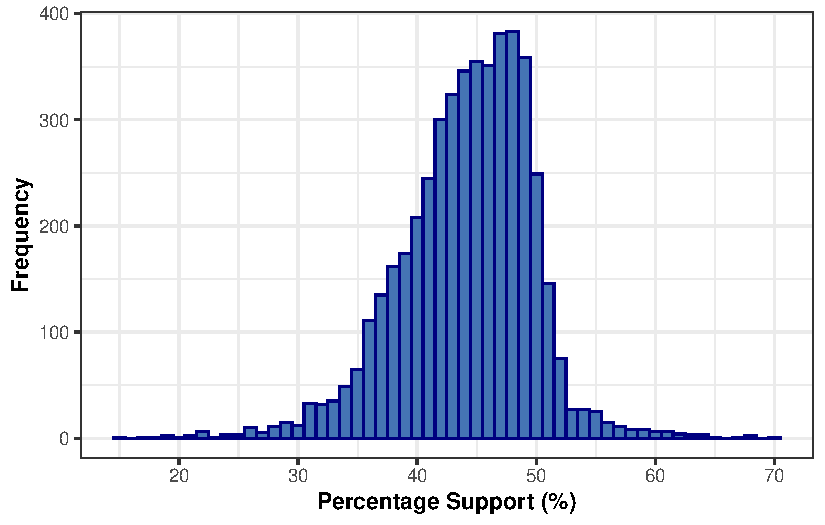
\includegraphics{Insights-and-Predictions-for-the-U.S.-Election_files/figure-pdf/fig-pct-1.pdf}

}

\caption{\label{fig-pct}Distribution of percentage support for Trump}

\end{figure}

\hypertarget{predictor-variables}{%
\subsection{Predictor variables}\label{predictor-variables}}

\hypertarget{summary-of-predictor-variables}{%
\subsubsection{Summary of Predictor
Variables}\label{summary-of-predictor-variables}}

\begin{itemize}
\item
  \textbf{State:} The U.S. state where the poll was conducted, if
  applicable.
\item
  \textbf{Numeric Grade:} A numeric rating from 0.0 to 3.0 indicating
  each pollster's reliability.
\item
  \textbf{Sample Size:} The total number of respondents participating in
  the poll.
\item
  \textbf{Poll Score:} A quantitative measure of the pollster's
  reliability, where lower values suggest higher predictive accuracy.
\item
  \textbf{Recency Weight:} A metric used to assess the relevance of
  polling data based on how close the polling dates are to an upcoming
  election. It is calculated by evaluating the number of days until the
  election from both the start and end dates of the poll, normalizing
  these values against the maximum days from other polls. The resulting
  weight gives more importance to more recent polling data, reflecting
  its greater influence on understanding current public sentiment..
\item
  \textbf{Candidate Name:} Indicate the corresponding presidential
  candidate. Trump was represented by 0, while Harris was represented by
  1.
\end{itemize}

\hypertarget{state}{%
\subsubsection{State}\label{state}}

According to Figure~\ref{fig-state}, we observe an interesting trend: in
traditionally Republican states, Trump's support is not markedly high
and is even relatively low in places like Oklahoma and Tennessee.
Conversely, in states typically aligned with the Democratic Party, as
well as in swing states, Trump's support is unexpectedly higher. The
``national'' category in the chart represents data spanning the entire
country without focusing on specific states, showing Trump's national
support nearing but not reaching 50\%. This suggests Trump's appeal may
be crossing traditional partisan lines, gaining unexpected traction
outside Republican strongholds. Overall, his estimated national support
stands at around 49\%, indicating a deeply divided electorate.

\begin{figure}

{\centering 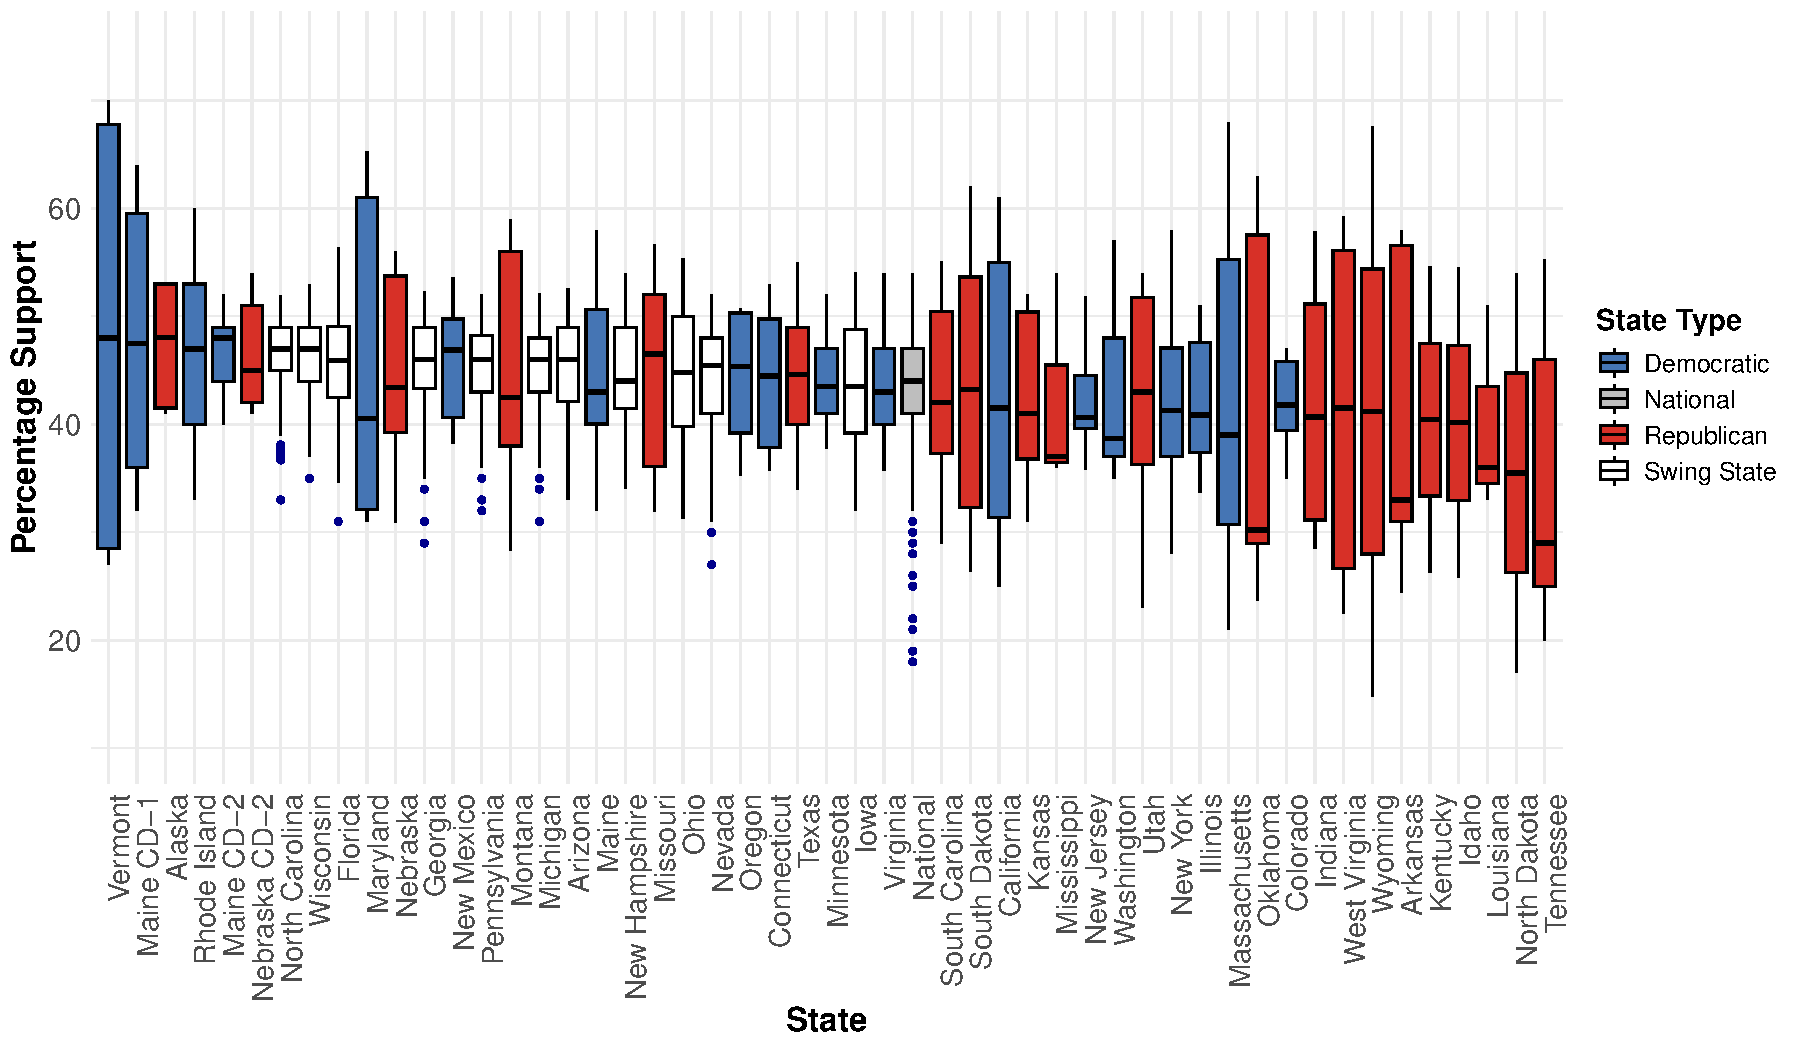
\includegraphics{Insights-and-Predictions-for-the-U.S.-Election_files/figure-pdf/fig-state-1.pdf}

}

\caption{\label{fig-state}Overview of the Percentage Support of Trump
Across Different States}

\end{figure}

\hypertarget{numeric-grade}{%
\subsubsection{Numeric Grade}\label{numeric-grade}}

In Figure~\ref{fig-method}, we analyzed the relationship between numeric
grade and Trump's support rate. Each point in the chart represents a
poll, with its numeric grade on the x-axis and Trump's support rate on
the y-axis. The nearly flat trend line suggests that numeric grade has
no clear relationship with Trump's support rate. However, this is a
basic analysis and does not rule out the possibility that numeric grade
could impact Trump's support rate under different variable conditions.

\begin{figure}

{\centering 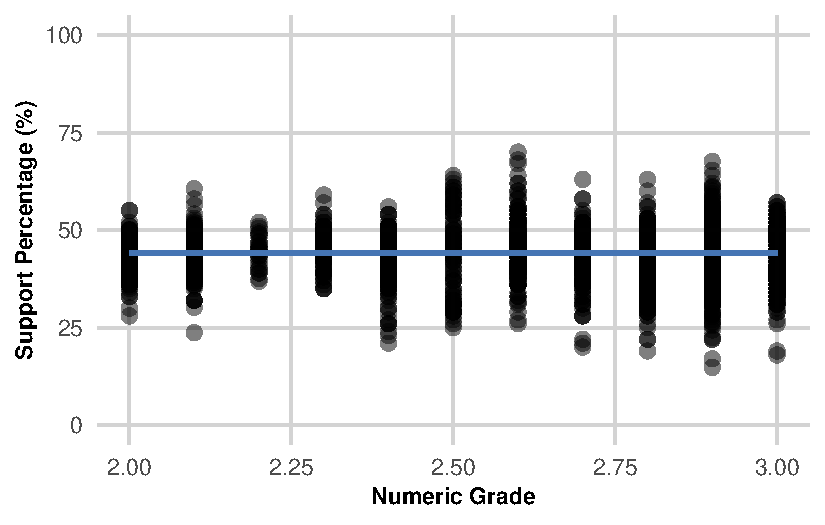
\includegraphics{Insights-and-Predictions-for-the-U.S.-Election_files/figure-pdf/fig-method-1.pdf}

}

\caption{\label{fig-method}Relationship between Numeric Grade and
Support Percentage of Trump}

\end{figure}

\hypertarget{sample-size}{%
\subsubsection{Sample Size}\label{sample-size}}

In Figure~\ref{fig-sample-size}, we examined the relationship between
sample size and Trump's support rate. The results show a slight downward
trend in Trump's support as sample size increases. However, since most
data points are concentrated in the 0--4000 range, with fewer data
points above 4000, this may not accurately reflect the true relationship
between sample size and support rate.

\begin{figure}

{\centering 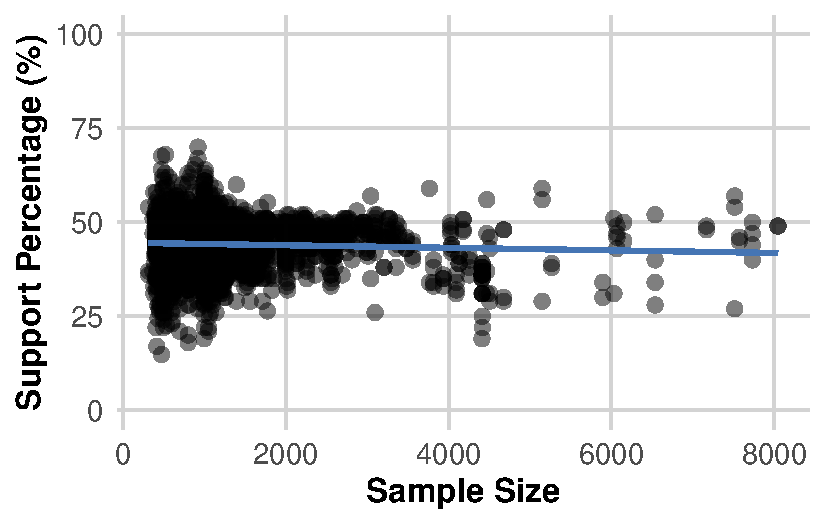
\includegraphics{Insights-and-Predictions-for-the-U.S.-Election_files/figure-pdf/fig-sample-size-1.pdf}

}

\caption{\label{fig-sample-size}Relationship between Sample Size and
Support Percentage for Trump}

\end{figure}

\hypertarget{poll-score}{%
\subsubsection{Poll Score}\label{poll-score}}

Analysis of Figure~\ref{fig-Pollscore} shows no clear proportional or
inverse relationship between poll scores and Trump's support rate. This
suggests that while a higher poll score may indicate greater
reliability, it does not directly translate into changes in candidate
support. This also supports the data's credibility, as Trump's support
rate remains consistent regardless of pollster ratings.

\begin{figure}

{\centering 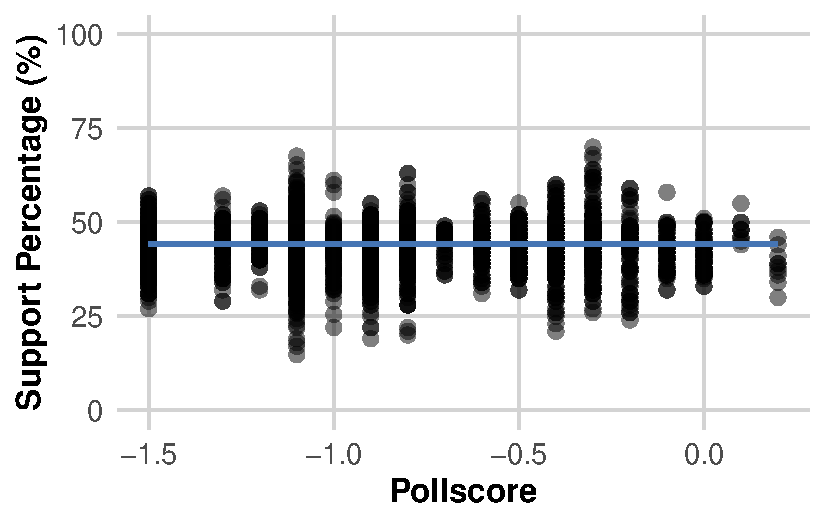
\includegraphics{Insights-and-Predictions-for-the-U.S.-Election_files/figure-pdf/fig-Pollscore-1.pdf}

}

\caption{\label{fig-Pollscore}Relationship between Pollscore and Support
Percentage of Trump}

\end{figure}

\hypertarget{recency-weight}{%
\subsubsection{Recency Weight}\label{recency-weight}}

Figure~\ref{fig-recency} shows the relationship between poll recency and
Trump's support rate. It indicates a slight upward trend in Trump's
support as polls get closer to Election Day, though the increase is not
significant.

\begin{figure}

{\centering 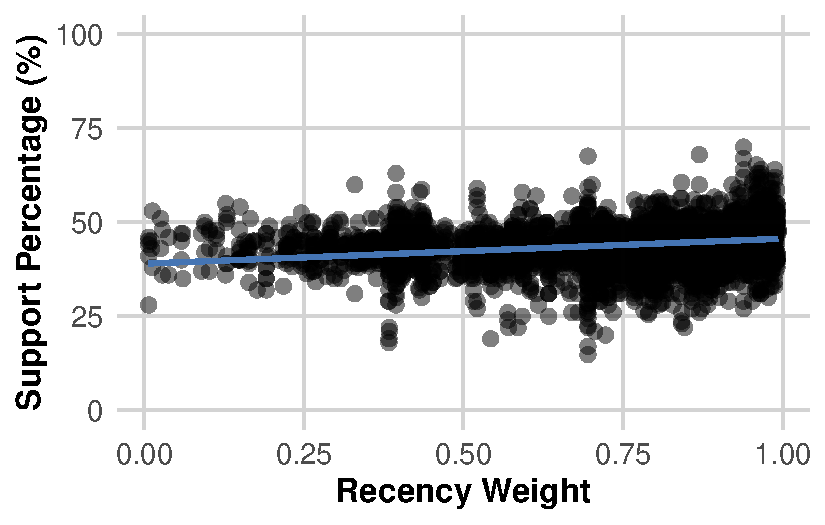
\includegraphics{Insights-and-Predictions-for-the-U.S.-Election_files/figure-pdf/fig-recency-1.pdf}

}

\caption{\label{fig-recency}Relationship between Recency Weight and
Support Percentage of Trump}

\end{figure}

\hypertarget{candidate-name}{%
\subsubsection{Candidate Name}\label{candidate-name}}

To predict Trump's probability of winning the election, we will create a
model containing the aforementioned predictor variables to forecast the
support rates for both Trump and his main opponent, Harris. To ensure
fairness in the results, we will use the same model to predict the
support rates for Trump and Harris. Thus, we have created a variable
called candidate\_name, where Trump is represented by a value of 0 and
Harris by a value of 1.

\hypertarget{sec-model}{%
\section{Model}\label{sec-model}}

The goal of this section is to address the inherent biases and
variations present in polling data to build a robust predictive model.
The key challenge lies in achieving an optimal balance between model
complexity and fit, ensuring that the model accurately captures the
dynamics of polling data while avoiding overfitting. To this end, we
evaluated multiple model specifications to identify the one that best
meets our forecasting objectives.

We chose to use ``numeric grade'' and ``poll score'' as variables
instead of ``pollster'' because ``pollster'' tends to be highly
subjective. People often select polling organizations that favor their
preferred candidate, which can introduce bias. In contrast, ``numeric
grade'' and ``poll score'' offer a more objective, quantified reflection
of poll quality and bias, helping to improve accuracy and reliability in
the regression analysis. Additionally, we focused on key factors such as
sample size, state, and recency, gradually adding complexity to the
model.

By systematically comparing model specifications that incorporate
different variables, we aim to identify a model that strikes the right
balance between predictive accuracy and generalizability, ultimately
providing the most reliable forecast results.

\hypertarget{model-set-up}{%
\subsection{Model set-up}\label{model-set-up}}

We aim to model the percentage of support for a candidate based on
factors such as candidate name, recency weight, state, sample size,
pollscore, and numeric grade. This model includes interaction terms to
capture how combinations of these factors jointly impact the support
percentage, providing a more comprehensive understanding of the
influences on candidate support.

\hfill\break
\begin{align*}
\mathrm{Pct}_i = &\ \beta_0 + \beta_1 \cdot \mathrm{Candidate Name}_i + \beta_2 \cdot \mathrm{Recency Weight}_i + \beta_3 \cdot \mathrm{State}_i \\
& + \beta_4 \cdot (\mathrm{Candidate Name}_i \times \mathrm{Recency Weight}_i) + \beta_5 \cdot (\mathrm{Candidate Name}_i \times \mathrm{State}_i) \\
& + \beta_6 \cdot (\mathrm{Recency Weight}_i \times \mathrm{State}_i) + \beta_7 \cdot (\mathrm{Candidate Name}_i \times \mathrm{Recency Weight}_i \times \mathrm{State}_i) \\
& + \beta_8 \cdot \mathrm{Sample Size}_i + \beta_9 \cdot \mathrm{Pollscore}_i + \beta_{10} \cdot \mathrm{Numeric Grade}_i + \epsilon_i
\end{align*}\\

Where

\begin{itemize}
\tightlist
\item
  \(y_i\) : the percentage of support for candidate in poll i,
\item
  \(\beta_0\): Intercept term, representing the predicted \texttt{pct}
  when all independent variables are 0.
\item
  \(\beta_1\): Main effect of \texttt{candidate\ name}, capturing the
  influence of the candidate.
\item
  \(\beta_2\): Main effect of \texttt{recency\ weight}, reflecting the
  influence of how recent the poll is on \texttt{pct}.
\item
  \(\beta_3\): Main effect of \texttt{state}, indicating the impact of
  different states on \texttt{pct}.
\item
  \(\beta_4\): Interaction effect between \texttt{candidate\ name} and
  \texttt{recency\ weight}, representing the combined influence of the
  candidate and recency of the poll.
\item
  \(\beta_5\): Interaction effect between \texttt{candidate\ name} and
  \texttt{state}, capturing the combined influence of the candidate and
  state.
\item
  \(\beta_6\): Interaction effect between \texttt{recency\ weight} and
  \texttt{state}, reflecting the joint impact of recency and state on
  \texttt{pct}.
\item
  \(\beta_7\): Three-way interaction between \texttt{candidate\ name},
  \texttt{recency\ weight}, and \texttt{state}, representing the
  combined effect of candidate, recency, and state.
\item
  \(\beta_8\): Main effect of \texttt{sample\ size}, showing the
  influence of sample size on \texttt{pct}.
\item
  \(\beta_9\): Main effect of \texttt{pollscore}, capturing the
  influence of the poll score on \texttt{pct}.
\item
  \(\beta_{10}\): Main effect of \texttt{numeric\ grade}, indicating the
  impact of the poll's numeric grade on \texttt{pct}.
\item
  \(\epsilon_i\): the error term, assumed to follow a normal
  distribution with mean 0.
\end{itemize}

\hypertarget{model-interpretation}{%
\subsubsection{Model interpretation}\label{model-interpretation}}

This regression model is designed to predict voter support rate by
incorporating a variety of factors and interaction terms. The model
includes an intercept term, representing the baseline support rate when
all other predictors are zero. Among the main effects, it includes terms
for candidate identity, poll recency, and state, capturing the influence
of these individual factors on support rate. For instance, candidate
identity indicates how different candidates affect voter support, poll
recency reflects how recent the poll is, and the state variable accounts
for regional variations in support.

To capture more complex relationships, the model incorporates two-way
interaction terms. These include interactions between candidate and
recency, candidate and state, and recency and state. Each of these terms
helps identify how one factor might alter the effect of another. For
example, the interaction between candidate and recency shows how the
influence of recency might differ for each candidate, while the
interaction between candidate and state captures how support for
different candidates varies by region. Additionally, the model includes
a three-way interaction term among candidate identity, poll recency, and
state, allowing it to account for combined effects that vary across
candidates, states, and the timing of the poll.

The model also includes several control variables, such as sample size,
poll score, and poll quality score. These variables help account for
variations in the data, with sample size ensuring that different poll
sizes are properly weighted, poll score reflecting potential bias within
each poll, and quality score indicating the reliability of each poll.
Finally, the model includes an error term to capture any unexplained
variation in support rate, adding robustness to its predictions.
Overall, this structure allows the model to incorporate both
straightforward and complex relationships, providing a nuanced and
reliable prediction of voter support.

\hypertarget{model-justification}{%
\subsection{Model justification}\label{model-justification}}

\hypertarget{tbl-model-compare}{}
\begin{longtable}[t]{l>{\raggedright\arraybackslash}p{8em}rrrrr}
\caption{\label{tbl-model-compare}Model Summary with Included Variables and Interactions }Model Summary with Included Variables and Interactions}\\
\toprule
Model & Variables & R² & Adjusted R² & AIC & BIC & RMSE\\
\midrule
Model 1 & Sample Size, Poll Score, Numeric Grade, State & 0.05260 & 0.04189 & 29535.84 & 29891.35 & 5.39274\\
Model 2 & Sample Size, Poll Score, Numeric Grade, State, Recency Weight & 0.09461 & 0.08417 & 29322.89 & 29684.86 & 5.27184\\
Model 3 & Sample Size, Poll Score, Numeric Grade, State, Recency Weight, Candidate Name & 0.09644 & 0.08583 & 29315.28 & 29683.71 & 5.26649\\
Model 4 & Candidate Name × State, Recency, Sample Size, Poll Score, Numeric Grade, State & 0.46417 & 0.45203 & 26938.52 & 27630.14 & 4.05562\\
Model 5 & Candidate Name × State × Recency, Sample Size, Poll Score, Numeric Grade, State & 0.48581 & 0.46410 & 26917.10 & 28171.08 & 3.97288\\
\bottomrule
\end{longtable}

Table~\ref{tbl-model-compare} summarizes the performance metrics for
five models, each with progressively more variables and interactions.

Model 1, which includes only basic predictors (Sample Size, Poll Score,
Numeric Grade, State), shows limited explanatory power, with an R² of
0.0526 and a high RMSE of 5.39274, indicating poor predictive accuracy.
Adding Recency Weight in Model 2 slightly improves performance,
increasing R² to 0.09461, but the RMSE remains high at 5.27184,
suggesting only minor gains in prediction accuracy. Model 3 further
incorporates Candidate Name, leading to a modest increase in R² to
0.09644, yet with minimal impact on RMSE (5.26649), indicating limited
additional explanatory value from this variable alone.

The inclusion of an interaction between Candidate Name and State in
Model 4 significantly enhances the model's fit, raising R² to 0.46417
and reducing RMSE to 4.05562. This improvement suggests that
state-specific variations in candidate popularity are important for
predictive accuracy. Finally, Model 5 builds upon Model 4 by adding a
three-way interaction among Candidate Name, State, and Recency Weight.
This final model achieves the highest R² (0.48581) and the lowest RMSE
(3.97288), indicating the best fit and prediction accuracy across all
models.

In conclusion, Model 5 is chosen as it captures complex interactions and
provides the best balance of explanatory power and prediction accuracy,
as evidenced by its highest R² and lowest RMSE.

\hypertarget{optimizatioit-will-not-be-mentioned-in-other-sections}{%
\subsection{Optimizatio(It will not be mentioned in other
sections)}\label{optimizatioit-will-not-be-mentioned-in-other-sections}}

Given that we identified the limitations of linear models in handling
interaction terms during our research, if we wish to investigate this
issue further, we propose an optimized model---Random Forest. The reason
we chose Random Forest over a linear model is because our data includes
interaction terms. Random Forest excels at handling interactions and
nonlinear relationships, as it can automatically identify and leverage
these complex interactions through its decision tree structure, without
requiring manual adjustments to the model structure. In contrast, linear
models have limited capabilities for handling interactions, typically
requiring manual specification and struggling to capture nonlinear
effects. Given that our data contains multiple interactions, Random
Forest can more flexibly adapt to the data structure, improving
prediction accuracy and model stability.

\hypertarget{tbl-rf}{}
\begin{longtable}[t]{lrr}
\caption{\label{tbl-rf}Predicted Average Percentages for Donald Trump vs.~Kamala Harris by
Random Forest }Predicted Percentage Vote for Donald Trump and Kamala Harris by Random Forest}\\
\toprule
Candidate Name & Average Predicted Percentage & Normalized Percentage\\
\midrule
\cellcolor{gray!10}{Donald Trump} & \cellcolor{gray!10}{44.54} & \cellcolor{gray!10}{50.42}\\
Kamala Harris & 43.80 & 49.58\\
\bottomrule
\end{longtable}

Table~\ref{tbl-rf} are the prediction results obtained through Random
Forest. Compared to a linear model, this result may be more accurate;
however, in the overall study, this method is only provided and will not
be the main subject of research.

\hypertarget{sec-results}{%
\section{Result}\label{sec-results}}

\hypertarget{tbl-trump}{}
\begin{longtable}[t]{rrrrrr}
\caption{\label{tbl-trump}Summary Statistics of Predicted Support for Donald Trump }Summary Statistics of Predicted Support for Donald Trump}\\
\toprule
Avg Support & Median Support & Min Support & Max Support & SD of Support & Total Polls\\
\midrule
\cellcolor{gray!10}{44.51} & \cellcolor{gray!10}{44.44} & \cellcolor{gray!10}{28} & \cellcolor{gray!10}{67.6} & \cellcolor{gray!10}{3.98} & \cellcolor{gray!10}{2248}\\
\bottomrule
\end{longtable}

Table~\ref{tbl-trump} shows the statistical information of the predicted
support rate for Trump. The average support rate is 44.51\%, with a
median of 44.44\%. The support rate ranges from a minimum of 28\% to a
maximum of 67.6\%. The standard deviation of the support rate is 3.98,
indicating some variability in the predictions. The data is derived from
2248 polls.

\hypertarget{tbl-modelresults}{}
\begin{longtable}[t]{lrr}
\caption{\label{tbl-modelresults}Predicted Average Vote Percentages for Donald Trump vs.~Kamala Harris }Predicted Percentage Vote for Donald Trump and Kamala Harris}\\
\toprule
Candidate Name & Average Predicted Percentage & Normalized Percentage\\
\midrule
\cellcolor{gray!10}{Donald Trump} & \cellcolor{gray!10}{44.51} & \cellcolor{gray!10}{50.37}\\
Kamala Harris & 43.86 & 49.63\\
\bottomrule
\end{longtable}

Table~\ref{tbl-modelresults} presents the model's average predicted vote
percentages for Donald Trump and Kamala Harris, along with their
normalized percentages. According to the model's predictions, Donald
Trump's average predicted vote percentage is 44.51\%, while Kamala
Harris's is 43.86\%. The normalized percentages adjust these predicted
values to relative proportions, with Donald Trump at 50.37\% and Kamala
Harris at 49.63\%. These results show that although Donald Trump's
average predicted vote percentage is slightly higher than Kamala
Harris's, the support rates for both candidates are nearly equal, with
Donald Trump holding a slight edge.

\begin{figure}

{\centering 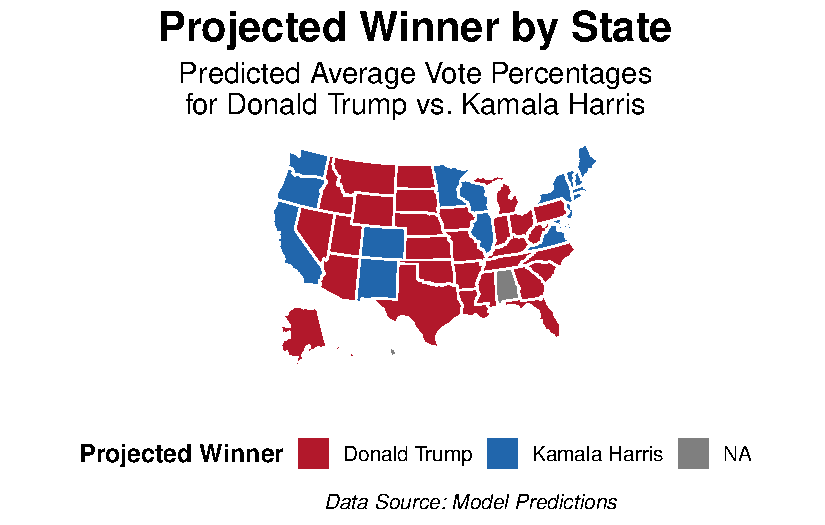
\includegraphics{Insights-and-Predictions-for-the-U.S.-Election_files/figure-pdf/fig-map-1.pdf}

}

\caption{\label{fig-map}Map of Projected Winner by State}

\end{figure}

Figure~\ref{fig-map} is a map showing the projected winner in each state
based on model predictions. Red indicates that Donald Trump is leading
in predicted support in that state, blue indicates that Kamala Harris is
leading, and gray signifies a lack of data for that state. Through this
map, readers can intuitively observe the regional support patterns for
both candidates across the nation. We can see that Donald Trump has an
advantage in some states in the Midwest and South, while Kamala Harris
performs better in parts of the Northeast and West. The following table
presents this data in tabular form.

\hypertarget{tbl-model-state}{}
\begin{longtable}[t]{lrrl}
\caption{\label{tbl-model-state}Table of Projected Winner by State }Predicted Average Vote Percentages and Projected Winner by State}\\
\toprule
State & Donald Trump (\%) & Kamala Harris (\%) & Projected Winner\\
\midrule
\cellcolor{gray!10}{Alaska} & \cellcolor{gray!10}{53.00} & \cellcolor{gray!10}{41.70} & \cellcolor{gray!10}{Donald Trump}\\
Arizona & 47.01 & 43.28 & Donald Trump\\
\cellcolor{gray!10}{Arkansas} & \cellcolor{gray!10}{57.30} & \cellcolor{gray!10}{29.47} & \cellcolor{gray!10}{Donald Trump}\\
California & 31.86 & 53.59 & Kamala Harris\\
\cellcolor{gray!10}{Colorado} & \cellcolor{gray!10}{38.52} & \cellcolor{gray!10}{44.44} & \cellcolor{gray!10}{Kamala Harris}\\
\addlinespace
Connecticut & 37.70 & 50.55 & Kamala Harris\\
\cellcolor{gray!10}{Florida} & \cellcolor{gray!10}{49.19} & \cellcolor{gray!10}{42.83} & \cellcolor{gray!10}{Donald Trump}\\
Georgia & 47.49 & 43.63 & Donald Trump\\
\cellcolor{gray!10}{Idaho} & \cellcolor{gray!10}{54.50} & \cellcolor{gray!10}{25.80} & \cellcolor{gray!10}{Donald Trump}\\
Illinois & 36.37 & 47.80 & Kamala Harris\\
\addlinespace
\cellcolor{gray!10}{Indiana} & \cellcolor{gray!10}{53.40} & \cellcolor{gray!10}{32.88} & \cellcolor{gray!10}{Donald Trump}\\
Iowa & 49.15 & 38.56 & Donald Trump\\
\cellcolor{gray!10}{Kansas} & \cellcolor{gray!10}{50.23} & \cellcolor{gray!10}{36.70} & \cellcolor{gray!10}{Donald Trump}\\
Kentucky & 54.60 & 26.30 & Donald Trump\\
\cellcolor{gray!10}{Louisiana} & \cellcolor{gray!10}{51.00} & \cellcolor{gray!10}{34.50} & \cellcolor{gray!10}{Donald Trump}\\
\addlinespace
Maine & 40.44 & 49.70 & Kamala Harris\\
\cellcolor{gray!10}{Maine CD-1} & \cellcolor{gray!10}{35.20} & \cellcolor{gray!10}{60.00} & \cellcolor{gray!10}{Kamala Harris}\\
Maine CD-2 & 47.00 & 46.40 & Donald Trump\\
\cellcolor{gray!10}{Maryland} & \cellcolor{gray!10}{32.46} & \cellcolor{gray!10}{58.85} & \cellcolor{gray!10}{Kamala Harris}\\
Massachusetts & 29.21 & 54.90 & Kamala Harris\\
\addlinespace
\cellcolor{gray!10}{Michigan} & \cellcolor{gray!10}{45.87} & \cellcolor{gray!10}{44.54} & \cellcolor{gray!10}{Donald Trump}\\
Minnesota & 42.29 & 46.01 & Kamala Harris\\
\cellcolor{gray!10}{Mississippi} & \cellcolor{gray!10}{54.00} & \cellcolor{gray!10}{36.50} & \cellcolor{gray!10}{Donald Trump}\\
Missouri & 52.31 & 37.10 & Donald Trump\\
\cellcolor{gray!10}{Montana} & \cellcolor{gray!10}{54.77} & \cellcolor{gray!10}{36.51} & \cellcolor{gray!10}{Donald Trump}\\
\addlinespace
National & 43.35 & 43.35 & Donald Trump\\
\cellcolor{gray!10}{Nebraska} & \cellcolor{gray!10}{53.26} & \cellcolor{gray!10}{37.84} & \cellcolor{gray!10}{Donald Trump}\\
Nebraska CD-2 & 41.89 & 51.11 & Kamala Harris\\
\cellcolor{gray!10}{Nevada} & \cellcolor{gray!10}{46.48} & \cellcolor{gray!10}{42.45} & \cellcolor{gray!10}{Donald Trump}\\
New Hampshire & 42.20 & 46.73 & Kamala Harris\\
\addlinespace
\cellcolor{gray!10}{New Jersey} & \cellcolor{gray!10}{38.50} & \cellcolor{gray!10}{46.17} & \cellcolor{gray!10}{Kamala Harris}\\
New Mexico & 41.04 & 49.84 & Kamala Harris\\
\cellcolor{gray!10}{New York} & \cellcolor{gray!10}{36.14} & \cellcolor{gray!10}{48.21} & \cellcolor{gray!10}{Kamala Harris}\\
North Carolina & 47.33 & 45.15 & Donald Trump\\
\cellcolor{gray!10}{North Dakota} & \cellcolor{gray!10}{54.00} & \cellcolor{gray!10}{17.00} & \cellcolor{gray!10}{Donald Trump}\\
\addlinespace
Ohio & 49.55 & 40.14 & Donald Trump\\
\cellcolor{gray!10}{Oklahoma} & \cellcolor{gray!10}{58.74} & \cellcolor{gray!10}{28.15} & \cellcolor{gray!10}{Donald Trump}\\
Oregon & 37.90 & 50.45 & Kamala Harris\\
\cellcolor{gray!10}{Pennsylvania} & \cellcolor{gray!10}{45.63} & \cellcolor{gray!10}{45.24} & \cellcolor{gray!10}{Donald Trump}\\
Rhode Island & 38.50 & 53.86 & Kamala Harris\\
\addlinespace
\cellcolor{gray!10}{South Carolina} & \cellcolor{gray!10}{50.72} & \cellcolor{gray!10}{37.46} & \cellcolor{gray!10}{Donald Trump}\\
South Dakota & 54.95 & 31.28 & Donald Trump\\
\cellcolor{gray!10}{Tennessee} & \cellcolor{gray!10}{47.66} & \cellcolor{gray!10}{24.50} & \cellcolor{gray!10}{Donald Trump}\\
Texas & 48.91 & 40.31 & Donald Trump\\
\cellcolor{gray!10}{Utah} & \cellcolor{gray!10}{51.29} & \cellcolor{gray!10}{33.23} & \cellcolor{gray!10}{Donald Trump}\\
\addlinespace
Vermont & 28.00 & 68.50 & Kamala Harris\\
\cellcolor{gray!10}{Virginia} & \cellcolor{gray!10}{41.59} & \cellcolor{gray!10}{44.89} & \cellcolor{gray!10}{Kamala Harris}\\
Washington & 37.37 & 49.34 & Kamala Harris\\
\cellcolor{gray!10}{West Virginia} & \cellcolor{gray!10}{57.15} & \cellcolor{gray!10}{25.25} & \cellcolor{gray!10}{Donald Trump}\\
Wisconsin & 46.04 & 46.15 & Kamala Harris\\
\addlinespace
\cellcolor{gray!10}{Wyoming} & \cellcolor{gray!10}{67.60} & \cellcolor{gray!10}{14.80} & \cellcolor{gray!10}{Donald Trump}\\
\bottomrule
\end{longtable}

Table~\ref{tbl-model-state} provides a more detailed numerical
representation of the predicted support percentages and projected
winners for each state. Table~\ref{tbl-model-state} complements
Figure~\ref{fig-map}, allowing for a more specific view of Trump and
Harris performance in each state.

\hypertarget{sec-discussion}{%
\section{Discussion}\label{sec-discussion}}

\begin{center}\rule{0.5\linewidth}{0.5pt}\end{center}

\hypertarget{limitation}{%
\subsection{Limitation}\label{limitation}}

Our analysis focuses exclusively on data related to Trump, which may
weaken the overall analysis. In organizing the data, we excluded
pollsters with low scores to enhance its credibility; however, this
approach resulted in a smaller sample size and reduced coverage. When
examining the relationship between state and percentage (PCT), we did
not integrate PCT with sample size for comparison. We believe that all
decisions made by the collective data should be treated equally,
regardless of sample size. This perspective has led to some
counterintuitive results, such as states where Trump's party is strong
giving him fewer votes. Additionally, a significant portion of our raw
data lacks exact state labels, which introduces errors in analyzing the
relationship between state and PCT, even after processing. Our analysis
focuses exclusively on data related to Trump, which may weaken the
overall analysis. In organizing the data, we excluded pollsters with low
scores to enhance its credibility; however, this approach resulted in a
smaller sample size and reduced coverage. When examining the
relationship between state and PCT, we did not integrate PCT with sample
size for comparison. We believe that all decisions made by the
collective data should be treated equally, regardless of sample size.
This perspective has led to some counterintuitive results, such as
states where Trump's party is strong giving him fewer votes.
Additionally, a significant portion of our raw data lacks exact state
labels, which introduces errors in analyzing the relationship between
state and PCT, even after processing.

\hypertarget{future-study}{%
\subsection{Future Study}\label{future-study}}

\begin{center}\rule{0.5\linewidth}{0.5pt}\end{center}

\newpage

\hypertarget{appendix-a.}{%
\section*{Appendix a.}\label{appendix-a.}}
\addcontentsline{toc}{section}{Appendix a.}

\hypertarget{overview-of-emerson-college-polling-methodology-october-23-25-2024}{%
\subsection{Overview of Emerson College Polling Methodology (October
23-25,
2024)}\label{overview-of-emerson-college-polling-methodology-october-23-25-2024}}

The Emerson College Polling conducted a survey from October 23 to 25,
2024, targeting 1,000 likely voters to investigate the differences in
support for various candidates. In this presidential election, 58\%
support former President Donald Trump, while 39\% support Vice President
Kamala Harris.

\hypertarget{population-frame-and-sample}{%
\subsection{Population, Frame, and
Sample}\label{population-frame-and-sample}}

In this context, the target population consists of likely voters in the
U.S. elections, defined by their likelihood to vote in the upcoming
elections and their voting history, both of which are self-reported in
the survey. The sampling frame specifically focuses on likely voters in
Montana, who were reached through a combination of cell phone contacts
provided by Aristotle and an online voter panel from CINT. The sample
consists of 1,000 likely voters randomly selected from the sampling
frame, with their status determined by a combination of voter history,
registration status, and demographic data, all of which are
self-reported. This methodology provides a balanced overview of Montana
voters' priorities, with a credibility interval of +/- 3\%.

\hypertarget{sampling-approach-and-its-trade-offs}{%
\subsection{Sampling Approach and its
trade-offs}\label{sampling-approach-and-its-trade-offs}}

Emerson College utilized a mixed-mode sampling approach for its poll of
likely voters in Montana. This strategy involved two main methods:
sending MMS text messages linked to an online survey using Aristotle's
voter lists and accessing a pre-screenedd, opt-in online panel from
CINT. The MMS method is efficient and cost-effective, allowing
participants to complete the survey at their convenience, which can
enhance response rates. The online panel broadens coverage to include
voters not reachable through text, capturing a wider demographic range
across the state. Together, these methods create a diverse sample while
reducing costs compared to traditional phone or in-person interviews.

However, this approach has trade-offs. The MMS survey requires
recipients to have active cell phones and internet, potentially
excluding older or less tech-savvy voters. Additionally, the online
panel consists of self-selected participants, which may not fully
reflect the general voter population. Mixing data from both sources can
introduce inconsistencies, as each method may attract different
respondent types, necessitating careful weighting to maintain balance
and accuracy. Smaller demographic subsets, such as age, race, or
education, carry higher credibility intervals due to reduced sample
sizes, limiting precision in analysis. Overall, the mixed approach
optimizes reach, reduces costs, and captures a representative snapshot
of Montana's voter priorities, albeit with some limitations.

\hypertarget{non-response-handling}{%
\subsection{Non-response Handling}\label{non-response-handling}}

Emerson College does not provide specific details regarding its
non-response management. While it mentions that data were weighted by
demographics such as gender, education, race, age, party registration,
and region to align with the 2024 likely voter model, this weighting
primarily addresses demographic imbalances and does not directly
mitigate non-response bias. The survey lacks information on common
non-response strategies, such as follow-up attempts, participation
incentives, or specific adjustments for non-responders. This absence
raises concerns about potential non-response bias, particularly if
certain demographic groups were less likely to engage with the survey.

\hypertarget{questionnaire-design}{%
\subsection{Questionnaire Design}\label{questionnaire-design}}

This questionnaire has strong points. Its straightforward and clear
wording makes questions easy for respondents to follow and reduces
potential confusion. By focusing on core issues like the economy,
housing, and voter approval for specific candidates, it captures key
voter concerns in Montana, offering a concise yet comprehensive view.
The use of multiple questions around candidate approval, voter issues,
and demographics adds depth and helps validate responses across topics.
However, the questionnaire also has limitations. While demographic
questions enhance the survey's representativeness, smaller groups (e.g.,
nonbinary individuals) may carry higher credibility intervals, reducing
precision for those subgroups. The mixed-mode approach (online panel and
mobile) improves access but still risks non-response bias, as certain
demographics might be less likely to participate. Overall, the design
achieves clarity and breadth, though response biases and sample
variations should be considered in interpreting the findings. For
example, in this survey of 1,000 Montana voters, only 5 respondents
identified as nonbinary or other genders. Since statistical reliability
depends on the number of responses, small groups have higher
variability, meaning their responses can swing widely due to each
individual answer carrying greater weight.

\hypertarget{appendix-b.}{%
\section*{Appendix b.}\label{appendix-b.}}
\addcontentsline{toc}{section}{Appendix b.}

\hypertarget{idealized-methodology-for-forecasting-the-u.s.-presidential-election}{%
\subsection{Idealized Methodology for Forecasting the U.S. Presidential
Election}\label{idealized-methodology-for-forecasting-the-u.s.-presidential-election}}

We aim to develop a methodology for forecasting U.S. presidential
election outcomes by conducting a survey with a \$100,000 budget. Using
stratified random sampling and multi-mode recruitment, the survey
targets 10,000 likely voters across demographic and regional lines. Key
measures include data validation checks, weighted analysis, and
predictive modeling to ensure accuracy. Results will be enriched by
aggregating reputable data sources like FiveThirtyEight for a
comprehensive, reliable forecast.

\hypertarget{budget-allocation}{%
\subsection{Budget Allocation}\label{budget-allocation}}

Funding allocations will focus on ensuring thorough and effective
sampling, recruitment, data validation, and analysis methods are
employed with a total budget of no more than \$10,000. The proposed
budget breakdown is as follows:

Survey platform costs: \$10,000 (subscription fees for online survey
tools such as Google Forms or Qualtrics) Respondent incentives: \$10,000
(gift cards or other incentives to encourage participation) Recruitment
and staffing: \$35,000 (staffing costs for survey distribution and data
collection) Data analysis tools: \$20,000 (statistical software
licenses, data cleaning and analysis) Marketing and promotion: \$10,000
(awareness and engagement campaigns) Contingency fund: \$5,000 (for
unexpected expenses)

\hypertarget{sampling-approach}{%
\subsection{Sampling Approach}\label{sampling-approach}}

The sampling approach will employ a stratified random sampling method to
ensure representation across various demographic groups, including age,
gender, race, education level, geographical location, and party
affiliation. The target population consists of likely voters in the
U.S., defined by historical voting behavior and self-reported intentions
to vote. A sample size of approximately 10,000 respondents will be aimed
at ensuring statistical robustness and a credibility interval of +/- 1\%
at a 95\% confidence level. This will be achieved through a combination
of national voter registration databases to identify potential
respondents. For example, we can utilize the National Voter Registration
Act (NVRA) data from the National Association of Secretaries of State
(NASS) to access information on registered voters. This database will
allow us to filter for likely voters based on their registration status
and historical voting behavior, ensuring that our sampling frame is
comprehensive and representative of the electorate. By leveraging such
reliable sources, we can create a sampling framework that enhances the
accuracy of our election forecasts.

\hypertarget{respondent-recruitment}{%
\subsection{Respondent Recruitment}\label{respondent-recruitment}}

To reach the target population, a multi-mode recruitment strategy will
be implemented: Online Surveys: Use Google Forms to distribute the
survey electronically. Telephone Surveys: Conduct live telephone
interviews to capture demographics that might not engage online. Text
Messaging Surveys: Implement SMS surveys to reach younger demographics
and those without regular internet access. Incentives: Offer gift cards
or other small incentives for participation, particularly for online
respondents. This can enhance response rates and engagement.

\hypertarget{data-validation}{%
\subsection{Data Validation}\label{data-validation}}

To effectively reach our target population and capture a diverse range
of perspectives, we will implement a multi-mode recruitment strategy
tailored to different demographic groups and communication preferences.
This approach includes online surveys using a Google Forms
questionnaire, which will be widely distributed through social media,
email lists, and community networks to maximize reach among individuals
who frequently engage online. The user-friendly platform allows
participants to complete the survey quickly and anonymously on any
internet-enabled device. The survey can be accessed through the
following link: \url{https://forms.gle/oSbad52Vuw9Z9Wf46}. Additionally,
we will conduct live telephone interviews to include participants who
may not be reachable through online channels, ensuring we capture
responses from populations that might otherwise be underrepresented. To
further engage younger demographics and individuals with limited
internet access, we will implement SMS-based surveys, allowing
participants to respond quickly via text. To encourage participation and
improve response rates, small incentives such as digital gift cards will
be offered, particularly for online respondents, with details
communicated at the survey's start and awarded upon completion to ensure
transparency. This comprehensive approach will enable us to gather a
robust and representative dataset, providing valuable insights into the
preferences and priorities of voters across multiple demographics.

\hypertarget{poll-aggregation-and-modeling}{%
\subsection{Poll Aggregation and
Modeling}\label{poll-aggregation-and-modeling}}

Poll results will be aggregated using statistical methods to identify
trends and analyze historical voting patterns. We will implement a
weighted analysis to ensure demographic representation, applying
specific weights based on factors such as age, gender, race, and
education level, as well as state significance to reflect regional
variations in voter behavior. Predictive analytics will primarily
involve logistic regression to model voting preferences and forecast
election outcomes, supplemented by time-series analysis to track changes
in voter sentiment over the campaign period. To enhance our findings, we
will combine our data with reputable sources like FiveThirtyEight,
utilizing their aggregation techniques to enrich our analysis with
broader insights.

\newpage

\hypertarget{references}{%
\section*{References}\label{references}}
\addcontentsline{toc}{section}{References}

\hypertarget{refs}{}
\begin{CSLReferences}{1}{0}
\leavevmode\vadjust pre{\hypertarget{ref-tellingstories}{}}%
Alexander, Rohan. 2023. \emph{Telling Stories with Data}. Chapman;
Hall/CRC. \url{https://tellingstorieswithdata.com/}.

\leavevmode\vadjust pre{\hypertarget{ref-janitor}{}}%
Firke, Sam. 2023. \emph{Janitor: Simple Tools for Examining and Cleaning
Dirty Data}. \url{https://CRAN.R-project.org/package=janitor}.

\leavevmode\vadjust pre{\hypertarget{ref-fivethirtyeight2024}{}}%
FiveThirtyEight. 2024. {``Dataset: US Presidential General Election
Polls.''}
\url{https://projects.fivethirtyeight.com/polls/data/president_polls.csv}.

\leavevmode\vadjust pre{\hypertarget{ref-rstanarm}{}}%
Goodrich, Ben, Jonah Gabry, Imad Ali, and Sam Brilleman. 2022.
{``{rstanarm: {Bayesian} applied regression modeling via {Stan}}.''}
\url{https://mc-stan.org/rstanarm/}.

\leavevmode\vadjust pre{\hypertarget{ref-lubridate}{}}%
Grolemund, Garrett, and Hadley Wickham. 2020. \emph{Lubridate: Make
Dealing with Dates a Little Easier}.
\url{https://CRAN.R-project.org/package=lubridate}.

\leavevmode\vadjust pre{\hypertarget{ref-ggmap}{}}%
McGlinn, Dale S., and Hadley Wickham. 2023. \emph{Ggmap: Spatial
Visualization in r}.
\url{https://cran.r-project.org/web/packages/ggmap/index.html}.

\leavevmode\vadjust pre{\hypertarget{ref-here}{}}%
Müller, Kirill. 2020. \emph{Here: A Simpler Way to Find Your Files}.
\url{https://CRAN.R-project.org/package=here}.

\leavevmode\vadjust pre{\hypertarget{ref-tibble}{}}%
Müller, Kirill, and Hadley Wickham. 2022. \emph{Tibble: Simple Data
Frames}. \url{https://CRAN.R-project.org/package=tibble}.

\leavevmode\vadjust pre{\hypertarget{ref-citeR}{}}%
R Core Team. 2023. \emph{{R: A Language and Environment for Statistical
Computing}}. Vienna, Austria: R Foundation for Statistical Computing.
\url{https://www.R-project.org/}.

\leavevmode\vadjust pre{\hypertarget{ref-gg2}{}}%
Wickham, Hadley. 2016. \emph{Ggplot2: Elegant Graphics for Data
Analysis}. \url{https://ggplot2.tidyverse.org}.

\leavevmode\vadjust pre{\hypertarget{ref-stringr}{}}%
---------. 2020. \emph{Stringr: Simple, Consistent Wrappers for Common
String Operations}. \url{https://CRAN.R-project.org/package=stringr}.

\leavevmode\vadjust pre{\hypertarget{ref-thereferencecanbewhatever}{}}%
Wickham, Hadley, Mara Averick, Jennifer Bryan, Winston Chang, Lucy
D'Agostino McGowan, Romain François, Garrett Grolemund, et al. 2019a.
{``Welcome to the {tidyverse}.''} \emph{Journal of Open Source Software}
4 (43): 1686. \url{https://doi.org/10.21105/joss.01686}.

\leavevmode\vadjust pre{\hypertarget{ref-tidy}{}}%
---------, et al. 2019b. {``Welcome to the {tidyverse}.''} \emph{Journal
of Open Source Software} 4 (43): 1686.
\url{https://doi.org/10.21105/joss.01686}.

\leavevmode\vadjust pre{\hypertarget{ref-knitr}{}}%
Xie, Yihui. 2023. \emph{Knitr: A General-Purpose Package for Dynamic
Report Generation in r}. \url{https://yihui.org/knitr/}.

\leavevmode\vadjust pre{\hypertarget{ref-kable}{}}%
Zhu, Hao. 2021. \emph{kableExtra: Construct Complex Table with 'Kable'
and Pipe Syntax}. \url{https://CRAN.R-project.org/package=kableExtra}.

\end{CSLReferences}



\end{document}
